\chapter{System Design and Implementation}
    \section{System Architecture}
    The Smart Energy Consumption Forecasting System operates through a multi-stage pipeline. The process begins with data collection from three primary sources: NEA Monthly Operation Reports (PDF files), Open-Meteo Weather API, and Nepal Holiday Calendar. The PDF extraction module parses tabular data from the reports using pdfplumber. Weather data is fetched through HTTP requests to the Open-Meteo API. The data processing module then cleans, merges, and transforms these datasets. Feature engineering creates predictive features including temporal variables, weather metrics, and lag features. Finally, machine learning models are trained and evaluated to produce energy demand predictions.

    \begin{figure}[ht]
        \centering
        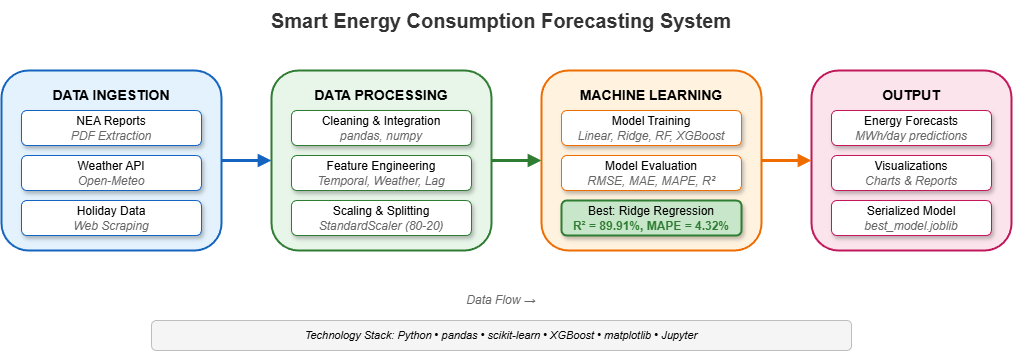
\includegraphics[width=0.95\textwidth]{img/System-Block-Diagram.png}
        \caption{System Architecture Block Diagram}
        \label{fig:System Block Diagram}
    \end{figure}

    \section{Data Collection Modules}

    \subsection{PDF Extraction Module}
    The PDF Extraction Module extracts tabular energy data from NEA Monthly Operation Reports using \textbf{pdfplumber}. The process involves:
    \begin{enumerate}
        \item Opening each PDF file from the data directory
        \item Iterating through pages to extract tables
        \item Parsing rows to identify daily energy and peak demand data
        \item Building DataFrames with standardized column names
    \end{enumerate}

    \textbf{Data Extracted:}
    \begin{itemize}
        \item Daily Energy Data: Date, Energy generation by source (NEA, NEA Subsidiary, IPP, Import), Total available, Export, Net demand met, Energy Interruption, Energy Requirement
        \item Peak Demand Data: Date, Peak time, Generation, Import, Availability, Demand
    \end{itemize}

    \subsection{Weather Data Module}
    Historical weather data is fetched from the Open-Meteo API (free, no API key required) for Kathmandu and Pokhara. Variables include:
    \begin{itemize}
        \item Temperature (mean, max, min)
        \item Relative humidity
        \item Precipitation
        \item Wind speed
    \end{itemize}
    Hourly data is aggregated to daily level for correlation with energy demand.

    \subsection{Holiday Calendar Module}
    Nepal's public holidays are compiled from timeanddate.com and hardcoded fallback data. Major festivals like Dashain and Tihar significantly impact energy consumption due to industrial shutdowns.

    \section{Feature Engineering}
    Feature engineering transforms raw data into predictive features:

    \subsection{Temporal Features}
    \begin{itemize}
        \item day\_of\_week, month, quarter, day\_of\_year, week\_of\_year
        \item season (Winter, Spring, Summer, Monsoon, Autumn based on Nepal's climate)
    \end{itemize}

    \subsection{Weather Features}
    \begin{itemize}
        \item temp\_mean, temp\_max, temp\_min, temp\_range
        \item humidity, precipitation, windspeed
    \end{itemize}

    \subsection{Lag Features}
    Lag features capture autocorrelation in energy demand:
    \begin{itemize}
        \item demand\_lag\_1: Previous day's energy demand
        \item demand\_lag\_7: Same day last week's demand
        \item demand\_rolling\_7: 7-day moving average
    \end{itemize}

    \subsection{Binary Flags}
    \begin{itemize}
        \item is\_weekend: 1 if Saturday or Sunday
        \item is\_holiday: 1 if public holiday
    \end{itemize}

    \section{Machine Learning Models}
    Four models were implemented and compared:

    \subsection{Linear Regression (Baseline)}
    Assumes linear relationship between features and target. Simple, interpretable, but may underfit complex patterns.

    \subsection{Ridge Regression}
    Adds L2 regularization to prevent overfitting. Handles multicollinearity well and is robust on small datasets.

    \subsection{Random Forest Regressor}
    Ensemble of decision trees using bagging. Captures non-linear relationships and provides feature importance. Parameters: n\_estimators=100, max\_depth=15.

    \subsection{XGBoost Regressor}
    Gradient boosting with regularization. State-of-the-art for tabular data. Parameters: n\_estimators=100, max\_depth=6, learning\_rate=0.1.

    \section{Evaluation Metrics}
    Model performance is evaluated using:
    \begin{itemize}
        \item \textbf{RMSE:} Root Mean Square Error - measures prediction error magnitude
        \item \textbf{MAE:} Mean Absolute Error - average absolute prediction error
        \item \textbf{MAPE:} Mean Absolute Percentage Error - percentage error for relative accuracy
        \item \textbf{R$^2$:} Coefficient of Determination - proportion of variance explained (closer to 1 is better)
    \end{itemize}

    \section{Model Persistence}
    Trained models are saved using joblib for future predictions:
    \begin{itemize}
        \item \texttt{models/best\_model.joblib} - Best performing model
        \item \texttt{models/scaler.joblib} - Feature scaler for standardization
    \end{itemize}